\chapter{改进从团队开始} % Introduction chapter suppressed from the table of contents

从下面两家美国公司五六十年代做改革的成功故事,让我们了解自主团队如何能带动公司提升。

但是这改进思路并非万事万能,后半部会总结背后的主要成功要素。

\hypertarget{ux7f8eux56fdux8d39ux57ce-weisbord-ux6545ux4e8b}{%
\subsection{美国费城 Weisbord
故事}\label{ux7f8eux56fdux8d39ux57ce-weisbord-ux6545ux4e8b}}

60 年代 复印机还未普及,很昂贵,所以为各类公司客户提供印刷服务就有市场,
这个故事的主人翁是某美国东岸一家印刷公司老板的儿子Weisbord。
他一直都没有接受什么正式的管理培训。 他有一个好朋友 Don
在国际大公司已工作了20 年, Don
推荐Weisbord说:``很多大公司已经开始推进团队自主管理,提升生产率, 
你可以先读 X-Y 理论(McGregor `Human side of Enterprise')一书。''

X 理论:

%\href{文件:0A_Agile_stories_p2.jpg}{文件:0A Agile stories p2.jpg}

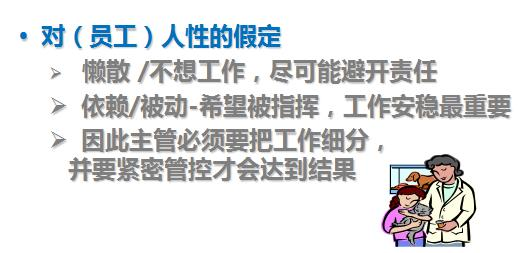
\includegraphics[width=6cm]{0A_Agile_stories_p2.jpg}

Y 理论:

%\href{文件:0A_Agile_stories_p3.jpg}{文件:0A Agile stories p3.jpg}

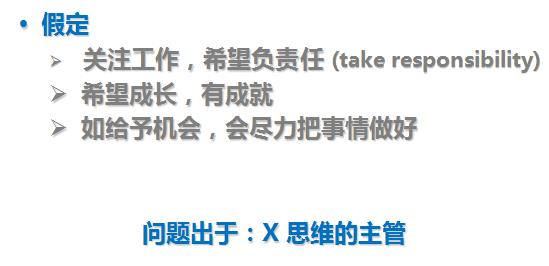
\includegraphics[width=6cm]{0A_Agile_stories_p3.jpg}

Weisbord
本来只想看看有多厉害,但他结果一口气一周末读完全书。他发现自己公司到处都是X
理论管理:

\begin{itemize}
\tightlist
\item
  工作分得很细,每员工不清楚全局
\item
  任务都是依赖主管分配
\item
  员工遇到问题、困难,交给主管处理
\item
  员工上下班打卡
\end{itemize}

他觉得这方式应该可以帮公司提升,但他担心单靠自己推动不了这个改革,
他便请Don过来正式加入公司。\\
他们分析公司业务最大问题是订单处理部门(Order Processing),
每个订单处理工作分到五、六个任务,员工只管被分配的任务,例如:

\begin{itemize}
\tightlist
\item
  筛选客户邮寄地址,邮寄印刷样本
\item
  输入订单
\item
  检查客户的信用
\item
  发起内部生产订单
\item
  用打字机打发票邮寄出去
\item
  收到的支票,对上那些应付账
\end{itemize}

公司平均每天要处理200 到300 个订单,
但因为工作分得很细,如果某个任务(如输入订单)有一、两人缺席,
便严重影响整个流程,效率会降低一半。\\
针对这问题,Weisbord 计划改革,把这部门的人分成多个4-5 人的团队,
把公司的两万个客户按地区分到各团队,每个团队有自己的客户名单,打字机等设备,
希望以此增加部门的灵活度,并提高生产率。\\
Weisbord 与5 位小主管(supervisor)商量,2 位很赞成,2 位中立,其他1
位觉得不会成功。 Weisbord 决策启动这改革,与Don 开始重组部门。\\

\hypertarget{ux5f00ux59cbux56e2ux961fux5236}{%
\subsubsection{开始团队制}\label{ux5f00ux59cbux56e2ux961fux5236}}

开始时问题非常多:

\begin{itemize}
\tightlist
\item
  B 物流公司运送出错,送到另一个城市,怎么办?
\item
  D 团队误解了生产的步骤,怎么办?
\item
  C 团队的样板工人,刚入职3 周,对我们公司产品线不熟识,怎么办?
\end{itemize}

原因很简单:本来每个人以前都只懂自己的一小块工作,以前问题都是由小主管处理。现在自主团队没有主管,都要靠团队自己想办法,像瞎子摸象。\\
但问题确实太多了,没办法,Don 建议每周开会讨论。
他们从未有每周开会的习惯,Weisbord
本来以为开会浪费时间,把时间用于生产更实际。
问题一直都非常多,延续了一个月。\\
Weisbord 开始怀疑这X-Y
理论,只是大学象牙塔里的玩意,难以真正用于实际公司环境。 Don
也没有更好的建议。\\
Weisbord 开始有撤销整个改革的想法,返回本来的组织架构, Don
还希望Weisbord 稍等一两周,看看有没有好转。但Weisbord
觉得一直这么多问题,严重影响公司运作,也难以与父亲交代,想在下次开会时向大家宣布变回本来架构。\\
到了第五周开会:\\
Weisbord,与以前开会一样,先问: 大家有什么问题?\\
沉默,几分钟后,某组长说:没有问题。\\
Weisbord:
为什么会没有?一直这么多问题(心里想,一定是你们也放弃了,连问题都不愿提了。)\\
另一组长回答:我们今周没有什么问题,遇到的问题都在以前的会议里面被解决了。\\

\hypertarget{ux6548ux679c}{%
\subsubsection{效果}\label{ux6548ux679c}}

改革的结果是从原来每天低于300
个订单提升到了400个。员工的出勤率也得到了改善,缺席率降低到接近零。\\
改革后的订单处理部平面图:

%\href{文件:0A_Agile_stories_p5.jpg}{文件:0A Agile stories p5.jpg}

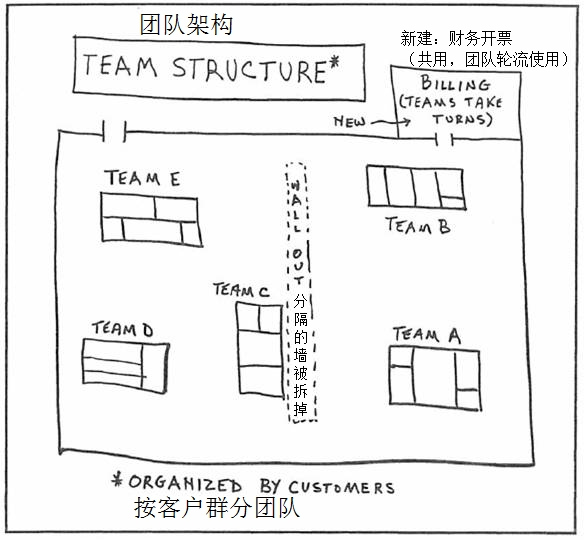
\includegraphics[width=6cm]{0A_Agile_stories_p51.jpg}

(团队自主改革前,小主管们为了减少各功能之间在处理订单引起的争吵,特意在中间加了一道墙;后面团队们一致建议把墙拆掉。)\\
Weisbord 
事后回顾:所有改变,重组都需要时间磨合,过程中管理者的支持非常重要,如果管理者不能坚持,面对并解决面对的困难,便会以失败告终。\\

\hypertarget{weisbord-ux6545ux4e8bux7684ux542fux53d1}{%
\subsection{Weisbord
故事的启发}\label{weisbord-ux6545ux4e8bux7684ux542fux53d1}}

如果员工具备知识技能,管理者便应尽力给员工平台,让团队自主发挥,才能不断提升竞争力,应对变化万千的市场需要,让员工与公司都受益;管理者不仅仅是制定目标、计划,发号施令的角色,而更应该是一位导师,辅助团队成长。\\
::= = = =
Lewin教授(心理学):``必须参与一起分析、讨论,才有动力后面采取行动。We
are likely to modify our own behavior when we participate in problem
analysis and solution, and likely to carry out discussions we have
helped
make.''这些实验也解释了为什么虽然Taylor先生科学管理本应可以提升工人的效率,但因为整个设计都是由专家设计,工人没有参与,所以反对。\\
Lewin 教授的实验与分析启发了随后的学者继续实验研究。

\hypertarget{ux7761ux8863ux5de5ux5382ux5b9eux9a8c-harwood-manufacturing}{%
\subsubsection{睡衣工厂实验 Harwood
Manufacturing}\label{ux7761ux8863ux5de5ux5382ux5b9eux9a8c-harwood-manufacturing}}

二战后,在维京尼亚州(Virginia),Harwood 是一家专门做睡衣的工厂。\\
难题:\\
要按不同的季节需求,做不同款式的睡衣,但往往有些女工习惯了某种工作方式,效率很高,但是要她改变工作方式,就接受不了,很难转换。

实验 - 比较三种变更方式:\\
*按传统方式,依赖工程师去设计每一轮的变更。团队只需要按设计去做。

\begin{itemize}
\tightlist
\item
  每个团队有代表与管理层去讨论如何变更,然后执行。
\item
  自己去策划自己的变更,也提建议。也安排那些女工每周跟那些生产率高和低的女工一起讨论不同方式的优劣,自己讨论怎么改变。
\end{itemize}

实验结果\\
*第一组按传统强制要求她们改变,花了3个月的时间,并引起很多不满,效果也不理想:生产率降低了百分二十,也发现有十个女工里面有一个后面就辞职不做了。

\begin{itemize}
\tightlist
\item
  第二组效果中等,需要大概两周才恢复到本来的水平。
\item
  第三组发现两天后就已经返回本来变更前的生产力水平,后面慢慢的上升提高到百分之十四。例如,某一个实验组就把本来一天45件,五天后提升到87件------一个本来无法想象的数字,后面甚至提到90件,超越本来那些工业工程师的目标。\\
\end{itemize}

这实验验证了集体讨论、自己管理,确实可以提升团队的生产率。结果也验证了实验前的发现:不同工人有自己不同的方式做事,没有像Taylor先生深信那种工作的最佳方式。\\

\hypertarget{ux7ed3ux8bba}{%
\subsubsection{结论}\label{ux7ed3ux8bba}}

问:这些故事是否想表达:我们就好比Taylor先生只是从工程方面去做优化。因为团队人员没有参与分析,导致他们难以接受和执行工程师(我们)设计的最佳方案。

答:你说得对。这些实验验证了群体行为:如果他们有参与或者可以影响结果,他们就有动力去做改进,如果要求他们听专家的最佳方案,往往就没有效果。五六十年代,越来越多公司采纳这个方式去做改进,也很多大学机构做这方面,培训不是用什么传统教学问的方式,而是用一些角色扮演或者团队的集体问题解决,去强调一个团队只要他们有收到及时的反馈,也比较开放,就可以做到一个民主的改进方式。下面另一个实验可以让我们更理解:

\framebox{%
\begin{minipage}[t]{0.97\columnwidth}\raggedright
自己做实验,取数据分析
一家工厂,很多主管都不愿意聘用三十岁以上的女工做机械操作工作,都觉得她们的生产力不如年轻女工高。你估计如果我们做顾问,给他一些数据,它会改变吗?不会。所以顾问只鼓励他们自己去做一些实验,证明那些三十岁的以上的女工确实生产率比年轻的低。他们确实按这个做了各种实验,但分析结果发现那些年纪大的女工无论生产力率,缺勤率、学习速度,更换工作流程的速率,都比年轻的好。后面他们也不再拒绝聘用年纪大的女工了。但其他那些没有参与做实验的团队,一直都不愿意改变。
\strut
\end{minipage}}


\hypertarget{ux7834ux51b0---ux53d8ux9769---ux7a33ux5b9a}{%
\subsection{破冰 - 变革 -
稳定}\label{ux7834ux51b0---ux53d8ux9769---ux7a33ux5b9a}}

以上两案例都可以归纳: 开始团队可以归纳:
自主团队管理都都需要经过下面三个阶段:\\
第一:破冰(Unfreezing),需要提供一些新的信息、新的数据,来减小/降低团队的反对声音。\\
第二:变革(Moving),要他们团队变态度、价值观、架构、行为等等。从以上的实验这个不能仅仅靠一些工程师去设计,最好是让他们自己讨论,得出他们觉得最合适的方式,他们才愿意按他们的讨论去执行。\\
第三:固定稳定下来(Refreezing)。当有了提升以后,需要有一些机制去维护新的行为方式,不要让它退回本来。与团队一起去研究、分析变成行动。顾问只是提供数据去破冰,减小反对的力量。所有变更、变革都会很痛苦、很困难。顾问或者公司管理层都应该有这些心理准备。例如本来的小组长、主管,他要接受在变更后角色的变化,不像以前是像将军一样继续下命令。

也类似过程改进戴明环(PDCA):\\
%\href{文件:IPM.png}{600px}

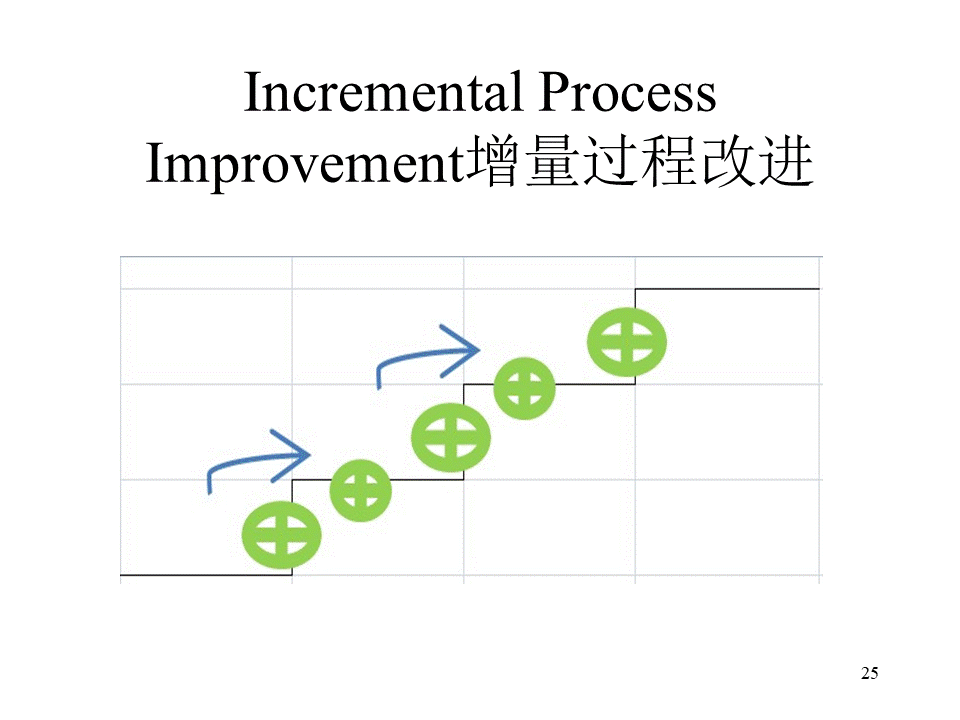
\includegraphics[width=6cm]{IPM.png}

从以上这些实验你应该也可以理解为什么本来Taylor先生那一套科学管理方式的不足。他只是考虑了工作方面、工程方面的因素,忽略了人性方面的考虑。但千万不要忽略工程方面的重要性。

\hypertarget{ux6210ux529fux8981ux7d20}{%
\subsection{成功要素}\label{ux6210ux529fux8981ux7d20}}

上面案例里的Weisbord
先生,后来卖掉了父亲创建的公司,自己成立顾问公司,他从六十年代开始做了几十家美国公司的改革,也发明了六个盒子方法
(Six-Box Model)。他的经验分享:\\
``每次跟企业做访谈、诊断时,一般顾问单是从公司遇到什么问题、什么困难、如何解决?跳出这个圈圈,从更高的角度去想这家公司有什么改进的潜力?有哪些人在公司里面可以持续推进这种改革?有没有一些让公司每个人都愿意参与的改进方向?那现在环境变化很快,顾问的角色应该是跳出为客户解决一些技术问题,诊断给药方,而是挖掘出员工的潜力,让他们动脑筋一起思考如何解决他们遇到的问题,才是一个对企业更有价值的东西。''\\
他建议要注意4个成功要素:

\hypertarget{ux516cux53f8ux6f5cux529b-assess-the-potential-for-action}{%
\subsubsection{公司潜力 Assess the Potential for
Action}\label{ux516cux53f8ux6f5cux529b-assess-the-potential-for-action}}

\textbf{Leadership commitment 领导支持}\\
这点最重要,顾问的责任不是诊断技术问题提供解决方案,更重要是探索公司有没有持续改进的潜力?如果缺乏的话,什么神医也医不了公司的病。

\begin{itemize}
\tightlist
\item
  有没有领导的支持?我接触很多公司,如果高层联系不上,或者不关心质量问题,觉得都可以委托他人解决,就很难做了。最常见就是老板是业务出身,一直都没有太关注软件工程,觉得写一个软件没有什么困难,市场和销售才最重要。反过来,如果有技术总监等,甚至软件工程质量的欠缺或者重要性,兴趣听可能的一些解决方案,这个公司才有潜力做一些持续改进。你可以想象如果我们开展培训,要求他们参加,如果高层不支持,后面什么都做不出来。下面的人也知道我们顾问,或者我们讨论后有什么建议、结果,老板或者高层也不关心,肯定就不会有什么效果。
\end{itemize}

\hypertarget{ux5546ux673a-good-business-opportunity}{%
\subsubsection{商机 Good Business
opportunity}\label{ux5546ux673a-good-business-opportunity}}

公司有没有一些持久的商机。在软件工程竞争很大,如果公司没有一些持久的方案、产品或者针对性。只是靠客户的关系接一些开发项目来做,就很难有一个长期的资源去投入,提升自己的质量。恰恰从我们的经验,这类软件开发公司会越来越难在这个市场上面竞争,比一些有能力、产品化的公司取代。

\hypertarget{ux5458ux5de5ux52a8ux529b-energized-people}{%
\subsubsection{员工动力 Energized
people}\label{ux5458ux5de5ux52a8ux529b-energized-people}}

公司里面有没有一些中层项目经理级别的人愿意投入时间,真心推动改革,原因是顾问只可以短时间帮助公司,长远还是要靠公司内部人员去推动。怎么识别有没有那些人呢?人可以分4种心态:如果是在下面两格的人的话
(Denial=否认 , Confusion=迷惑
),就不用想会支持这种变革,首先必须要是在上面的两格(Contentment=满足 ,
Renewal=更新) 
。所以作为顾问,你要识别有没有这种人,在公司里面要辅助他们作为整个公司改革变化的重要种子。\\
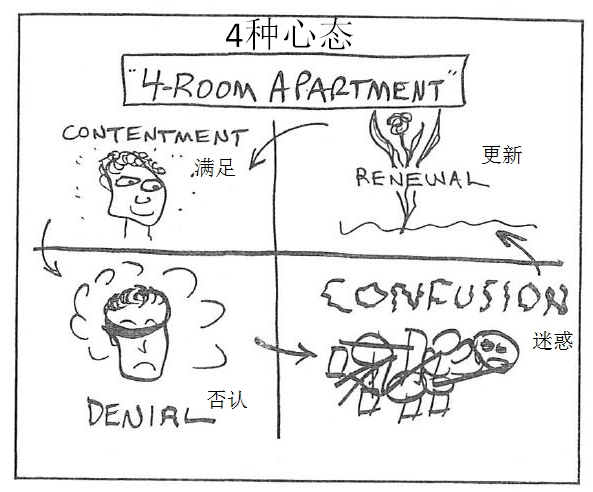
\includegraphics[width=6cm]{P335_4_room_apartment1.jpg}

\textbf{4种心态 与 对策:}

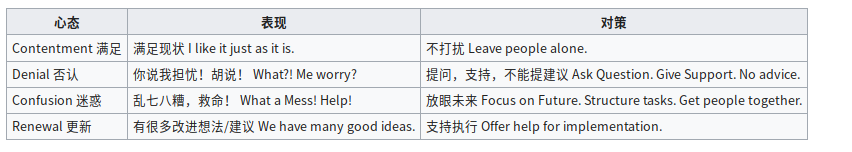
\includegraphics[width=6cm]{Screenshotfrom2023-11-0304-11-55.png}

注意: 人的心态会不断(按环境)循环变化。

\hypertarget{ux6280ux672fux521bux65b0-pocket-innovation}{%
\subsubsection{技术创新 Pocket
Innovation}\label{ux6280ux672fux521bux65b0-pocket-innovation}}

软件工程在技术方面变化很大,从我接触的公司,如果一直都没有使用一些新的技术平台,这类公司可以改进的机会极低。反过来,如果公司在过去做过一些内部的改进,比如引进一些自动化技术,推行持续交付、自动化测试等等,就看到这个公司其实已经在技术方面有很多不断提升、完善的项目在进行中,这个文化就更容易推动所有人参与、改进整个系统的可能性。\\

\hypertarget{ux7ed3ux675fux8bed}{%
\subsection{结束语}\label{ux7ed3ux675fux8bed}}

过程,改进需要每一个部门都参与,才可以提升公司的最终目标,公司是一个系统,所有员工参与改进整个系统:

%\href{文件:微信截图_20231025084623.png}{600px\textbar{}无}

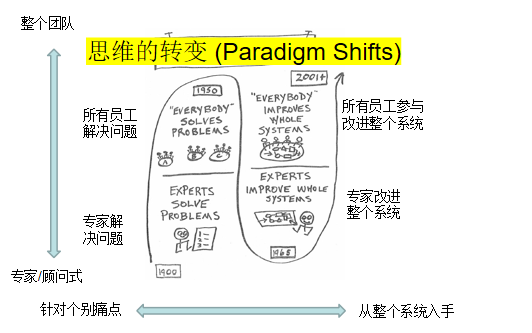
\includegraphics[width=6cm]{微信截图_20231025084623.png}

(上图参考 M. Weisbord, Productive Workplaces Revisited)

如果没有按照上面说的步骤,形成具体行动计划,很难取得效果。

过程改进不是一两个月、两三个月就出成绩,开始时候,员工可以关于创新、改进有想法,写文章分享,但要这个作为习惯继续下去,是需要有些新的想法和思路,这可以借助公司内部培训,比如有没有过程域相关的参考资料,内部分享会,学习小组,定期有老师的辅助指导,定期体检、诊断。


\hypertarget{ux9644ux4ef6}{%
\section{参考 References}\label{ux9644ux4ef6}}

\begin{enumerate}
\tightlist
\item
  McGregor, D.: \emph{The Human Side of Enterprise},1960.\\
\item
  Weisbord, M.R.: \emph{Productive workplaces revisited : dignity,
  meaning, and community in the 21st century}, 2004.
\end{enumerate}



